\chapter{The Language of Quantum Information Theory}
This chapter constructs the formalism for the study of open quantum systems we use in the rest of the thesis, in analogy with the
Quantum Mechanics (QM) postulates we demand that it must stablish two things: how this class of systems evolve and how to obtain its measurement
statistics, furthermore, it must follow from the postulates. To achieve the first one we introduce the notions of \textbf{system-enviroment scheme}, \textbf{marginalization}, and
\textbf{mixed state} by modeling them via Hilbert Spaces with tensor product structure, the partial trace and density operators, then these
are coupled with the unitary evolution postulate and lead us to the idea that all possible physical transformation in QM can be understood as a
special class of superoperators called \textbf{Quantum Operations} for which a few key results are presented.
\\\\
The second point is
obtained by realizing that measurements as precribed in the postulates are a valid type of quantum operation and when considered
as acting only on a subsystem lead to the notion of \textbf{generalized measurement}, which resembles much more how an actual measurement is
performed in a laboratory, and eventually allows us to show that all the information about the statistics is captured by
a set of positive operators called a \textbf{Positive Operator Valued Measure}.
% Section on density operator
\section{Density Operators}
%%%%%%%%%%Postulates of Quantum Mechanics
\subsection{Postulates of Quantum Mechanics}
We begin by stating the a common axiomatization of QM based on Hilbert Spaces following \cite{ballentine_quantum_2014}, we choose it for mathematical simplicity; for alternatives see e.g. \cite{reyes-lega_aspects_2015}.
\begin{enumerate}
        \item To each physical system $\mathcal{S}$ there corresponds a separable Hilbert Space $\mathcal{H}$ such that states of the system are described by positive and unit trace operators on it. The Hilbert Space of a composite system made up of $\mathcal{S}$ and $\mathcal{S}'$
        is given by the tensor product of the Hilbert spaces $\mathcal{H}\otimes\mathcal{H}'$.
        \item To each dynamical variable there corresponds a self-adjoint operator on $\mathcal{H}$, called an observable, whose possible
        values are given by its eigenvalues.
        \item Given a system in  state $\rho$ and some observable $A$ of it, the probability of measuring $A$ and obtaining the result
        $\lambda$ is given by $\mathrm{Tr}[\rho P_{\lambda}]$ where $P_{\lambda}$ is the eigen-projector into the subspace associated with
        $\lambda$. Furthermore the expectation value is $\mathrm{Tr}[\rho A]$.
        \item After a measurement with result $\lambda$ the state of the system becomes $\frac{P_{\lambda}\rho P_{\lambda}}{\mathrm{Tr}[P_{\lambda}\rho
        P_{\lambda}]}$.
        \item The time evolution of the system in a time interval $(0,t)$ in which no measurement is done is given by some unitary operator
        $U_{t}$ according to $\rho_{t}=U_{t}\rho U_{t}^{\dagger}$ where $\rho$ is the state of the system at time $t=0$.
\end{enumerate}
Operators satisfying the properties required for a state are called \textit{\textbf{Density Operators}} and in contrast to frameworks
whose treatment of quantum states is merely as rays in $\mathcal{H}$, they describe statistical mixtures so imperfect state preparation
can be handled. To see this consider the spectral resolution of some density operator:
\begin{equation}
  \rho = \sum_{n}p_{n}\ketbra{\psi_{n}}
\end{equation}
by definition we have $p_{n}\geq 0, \sum_{n}p_{n}=1$  any density operator can be seen as a convex sum of rays in $\mathcal{H}$ (provided we
identify each one with its associated projector $\ketbra{\psi}$) and from it an  interpretation of $\rho$ as an statistical mixture of rays is
suggested: given a preparation process, there is a probability $p_{n}$ for the system to be in the state $\ketbra{\psi_{n}}$ after it, for this
reason states of the form $\ketbra{\psi}$ are called \textbf{\textit{Pure}} while those who are not we refer to as \textbf{\textit{Mixed}}.
This \textbf{\textit{Ensemble Interpretation}} has serious conceptual challenges when one tries to use it outside a
fixed preparation procedure due to the non-uniqueness of the decomposition into pure states \cite{nielsen_quantum_2010},
but is good enough for the porposes of the present work, for a comprehensive discussion of this
topic the reader is refered to \cite{schlosshauer_decoherence_2007}.
%%%%%%%%%%%%%%Time evolution
\subsection{Time Evolution}
Assuming the evolution to be differentiable in time, we have that there exists a self-adjoint operator $H$ such that $U_{t} = \mathrm{exp}(-itH)$
\footnote{Unless otherwise stated, from here on we assume $\hbar=1$}, called the \textbf{\textit{Hamiltonian}} of the systems and which
acts as the generator of the dynamics. It is straightforward now to construct a differential equation for $\rho_{t}$ by taking the derivative
of it:

\begin{align}
  \rho_{t}=& e^{-itH}\rho_{t}  e^{itH}\\
  \partial_{t}\rho_{t} =& -iH\rho_{t} + \rho_{t}iH\\
  \partial_{t}\rho_{t} =& -i[H, \rho_{t}]\label{eq:Liouville-VonNeumann}.
\end{align}
Equation \eqref{eq:Liouville-VonNeumann} is called the Liouville-Von Neumann equation, it generalizes the  Schr\"{o}dinger equation
to mixed states and can be interpreted as the quantum analog of the Liouville equation in classical mechanics (with the Poisson braket) through
the quantization rule $\{\bullet,\bullet\} \to -i[\bullet,\bullet]$. As will be seen in later chapters, this type of evolution is characteristic
of closed quantum systems.
%%%%%%%%%%Purity
\subsection{Purity}
Say we got a particular state production processes whose product $\rho$ we characterize via say tomography \cite{nielsen_quantum_2010}, it
becomes immedeatley important to quantify to which extent we can regard the product as being composed of only one pure states
(hopefully the one we wanted to prepare) i.e. we want to define the purity of the state, with this motivation one look for a map
$\mathcal{E}$ from the space of density operators to the reals such that:
\begin{itemize}
        \item $\mathcal{E}(\rho)$ is maximal if and only if $\rho$ is pure.
        \item it is conserved under unitary evolution.
\end{itemize}
The first one makes this map a figure of merit one can try to maximize and the second one is imposed to assure that it doesn't changes in a
closed system unless a measurement is made, as allowing the free evolution of the system should not improve the knowledge of the
experimenter about the system. The standard choiche (altough not the only one) is the \textit{\textbf{Purity}},
defined as \cite{nielsen_quantum_2010, ballentine_quantum_2014}:
\begin{definition}
The purity $\gamma$ of a state $\rho$ is:
  \begin{equation}
    \gamma = \Tr{\rho^{2}}.\label{eq:definition_purity}
  \end{equation}
\end{definition}
The requirements are quickly checked:
\begin{align}
  \Tr{\rho^{2}_{t}} =& \Tr{(U_{t}\rho_{0}U_{t}^{\dagger})(U_{t}\rho_{0}U_{t}^{\dagger})} = \Tr{\rho_{0}^{2}}\\
  \Tr{\rho^{2}} =& \sum_{n}p_{n}^{2} \leq 1
\end{align}
in the second line the inequality is saturated if and only if $\rho=\ketbra{\psi}$.
\section{Entanglement}
One of the key differences between the structure of the state space of classical and quantum systems is the existance
of non-separable states when considering multipartite systems \cite{reyes-lega_aspects_2015,diosi_short_2011,nielsen_quantum_2010} which allows
the latter to have new a new type of correlations. Here we define entanglement for mixed states following \cite{diosi_short_2011}:

\begin{definition}
  Given a state $\rho$ in a system composed of two subsystems $A$ and $B$ with total Hilbert space $\mathcal{H}_{A}\otimes \mathcal{H}_{B}\}$, we say it is
  an \textbf{\textit{entangled}} or \textit{\textbf{non-separable}} if there doesn't exists a set states $\{\rho_{j}\otimes \sigma_{j}\}_{j}$ and coefficients
  $\{p_{j}\}_{j},  \sum_{j}p_{j}=1, \hspace{0.1cm} p_{j}\geq 0$ such that:
  \begin{equation}
    \rho = \sum_{j}p_{j}\rho_{j}\otimes \sigma_{j}
  \end{equation}
  if it does exists, the state is called \textbf{\textit{separable}}.
\end{definition}
For the case of pure state this definition coincides with the usually given one \cite{nielsen_quantum_2010}: say $\rho=\ketbra{\psi}$ is pure and separable, then:
\begin{equation}
  \Tr{\rho^{2}} = \sum_{jk}p_{j}p_{k}\Tr{\rho_{j}\rho_{k}}\Tr{\sigma_{j}\sigma_{k}}
\end{equation}
and by the Cauchy-Schwartz inequality with the Frobenious inner product
\begin{equation}
  \Tr{\rho^{2}} \leq \sum_{jk}p_{j}p_{k}\Tr{\rho_{j}^{2}}\Tr{\rho_{k}^{2}}\Tr{\sigma_{j}^{2}}\Tr{\sigma_{k}^{2}} \leq 1
\end{equation}
the first inequality from right to left saturates if and only if all the $\rho_{j}$ and $\sigma_{k}$ are pure, and the first one if
and only if all the $\rho_{j}$ and $\sigma_{k}$ are equal between themselves i.e. $p_{j}=\delta_{0j}$, hence there are pure states
in $\mathcal{H}_{A}$ and $\mathcal{H}_{B}$ such that:
\begin{equation}
  \ketbra{\psi} = \ketbra{\alpha}\otimes\ketbra{\beta}.
\end{equation}
For a classical system all states are separable thanks to the representation via $\delta$ functions
of probability densities \cite{diosi_short_2011} and in this sense entanglement is a purely non-classical phenomena, in fact for pure states
this completely exhaust all the possible non-classical correlations. For mixed states the characterization is considerably richer
and allows for bipartite states that despite being separable show non-classical correlations \cite{adesso2016introduction}.
\subsection{Marginalization}
Consider a bipartite system in state $\rho$ with subsystems $A$ and $B$, and assume only the former can be accessed
experimentally; e.g. $B$ is on the other side of the galaxy, has too many degrees of freedom or is simply not of interest and is desirable
to prescend from it. Any
observable $\Gamma$ that we decide to measure must be of the form $\Gamma=\Lambda \otimes I$ so that it describes only actions on
$\mathcal{H}_{A}$; in this sense we say it is \textit{\textbf{local}}. We want to obtain the probability distribution describing the statistics
of $\Lambda$, by definition:
%%%%%%%%%%%%%%%%%%%%%%%%%%%%%%%%%%%%%%%%%%HEREEEEEEE%%%%%%%%%%%%%%%%%%%%%%%%%%%%%%%%
 \begin{align}
   \wp(\lambda)=&\Tr{\rho (\ketbra{\lambda^{A}}\otimes I)}\\
   \wp(\lambda)=& \sum_{\lambda'k}\bra{\psi_{k}^{B}}\bra{\lambda^{'A}}\rho (\ketbra{\lambda}\otimes I)\ket{\lambda^{'A}}\ket{\psi_{k}^{B}}\\
    \wp(\lambda)=& \sum_{\lambda'k}\bra{\psi_{k}^{B}}\bra{\lambda^{'A}}\rho \ket{\lambda^{'A}}\ket{\psi_{k}^{B}} \delta_{\lambda\lambda'}\\
    \wp(\lambda)=& \sum_{k}\bra{\psi_{k}^{B}}\bra{\lambda^{A}}\rho \ket{\lambda^{A}}\ket{\psi_{k}^{B}} \\
    \wp(\lambda)=& \bra{\lambda^{A}} \left(\sum_{k}\bra{\psi_{k}^{B}}\rho\ket{\psi_{k}^{B}}\right)\ket{\lambda^{A}}\\
    \wp(\lambda)=& \Tr{\ketbra{\lambda^{A}}\sum_{k}\bra{\psi_{k}^{B}}\rho\ket{\psi_{k}^{B}}} \label{eq:partial_trace}.
 \end{align}
%%%%%%%%%%%%%%%%%%%%%%%%%%%%%%%%%%%%%%%%%%HEREEEEEEE%%%%%%%%%%%%%%%%%%%%%%%%%%%%%%%%
Equation \eqref{eq:partial_trace} suggest that there exists a state in $\mathcal{H}_{A}$ whose statistics  coincide
with those of $\rho$ and that it should be given by the sum in \eqref{eq:partial_trace}, in this sense we have a marginalization i.e.
an assignement of states of in $\mathcal{H}_{A}\otimes\mathcal{H}_{B}$ to states in $\mathcal{H}_{A}$ such that it has the correct statistics
i.e. $\Tr{\rho^{AB}(\Lambda \otimes I)}=\Tr{\rho^{A}\Lambda}$ for any observable $\Lambda$ of $A$. It is desirable for this map to be unique
for the following: assume an experimentalist has an infinite ensemble of copies of the system in state $\rho$ but can only measure local
observables in $A$, although any and as many time as wanted, i.e. it is possible to fully characterize the statistics of any local observable,
which state should the experimentalist asign? If the marginalization is not unique there is an ambiguity, an marginalizations sure must
exists as local experiments are always possible, hence uniqueness is important to account properly for this experiment; turns out to
assure it suffices to demand linearity. This map is called the \textit{\textbf{Partial Trace}}:

\begin{definition}
  Given two vector spaces $V$ and $W$, for simplicity assumed of finite dimension\footnote{although we will use it too for infinite dimensions without inquiring wheter the operators are even traceclass}, the partial trace taken over $W$ is the map\cite{nielsen_quantum_2010}:
\[
\mathrm{Tr}_{W}: \begin{array}{rcl}
A\otimes B \in \mathcal{L}(V\otimes W)& \mapsto & A \Tr{B} \in \mathcal{L}(V)
\end{array}
\]
where the $\mathcal{L}$ denotes the space of operator, and the map is  linearly extended to all of $\mathcal{L}(V\otimes W)$
.
\end{definition}
The linear extension makes the partial trace coincide with the sum in \eqref{eq:partial_trace} and the non-manifestly base invariant definition
usually given in sources like \cite{maziero2017computing}. Next we prove this is in fact the only linear map with the correct statistics:
\begin{theorem}
  The partial trace is the only linear map such that $\mathcal{E}:\to \mathcal{L}(\mathcal{H}_{A}\otimes \mathcal{H}_{B}) \to \mathcal{L}(\mathcal{H}_{A})$
  such that $\Tr{\rho (\Lambda\otimes I)} = \Tr{\mathcal{E}(\rho)\Lambda}$ for all $\rho \in \mathcal{H}_{A}\otimes \mathcal{H}_{B}$ and
  $\Lambda \in \mathcal{L}(\mathcal{H}_{A})$.
\end{theorem}
\begin{proof}
  Assume there exists a map $\mathcal{E}:\to \mathcal{L}(\mathcal{H}_{A}\otimes \mathcal{H}_{B}) \to \mathcal{L}(\mathcal{H}_{A})$ with the
  correct statistics and introduce an orthogonal product basis in $\mathcal{H}_{A}\otimes \mathcal{H}_{B}$,
  $\{\ket{\psi^{A}_{j}}\ket{\psi^{B}_{k}}\}_{jk}$. By construction we have:
  \begin{align}
    \Tr{\mathcal{E}(\rho)\Lambda} =& \sum_{jk} \bra{\psi^{B}_{j}}\bra{\psi^{A}_{k}}\rho (\Lambda \otimes I) \ket{\psi^{A}_{k}}\ket{\psi^{B}_{j}}\\
 \Tr{\mathcal{E}(\rho)\Lambda} =& \sum_{k} \bra{\psi_{k}^{A}}\sum_{j}\bra{\psi^{B}_{j}}\rho\ket{\psi^{B}_{j}}(\Lambda \ket{\psi_{k}^{A}})\\
\Tr{\mathcal{E}(\rho)\Lambda} =& \sum_{k} \bra{\psi_{k}^{A}}\Trp{B}{\rho}(\Lambda\ket{\psi_{k}^{A}})\\
\Tr{\mathcal{E}(\rho)\Lambda} =& \Tr{\Trp{B}{\rho}\Lambda}\\
  \end{align}
  As this holds for any $\Lambda$ and $\rho$, we have that $\mathcal{E}=\mathrm{Tr}_{B}$.
\end{proof}
Note that in the above proof we have not used any properties of $\rho$ or $\Lambda$ unlike in \eqref{eq:partial_trace}. A few remarks are
in order:
\begin{enumerate}
  \item The partial traces of an state $\rho \in \mathcal{L}(\mathcal{H}_{A}\otimes\mathcal{H}_{B})$ are always mixed, unless $\rho$ is
        both pure and separable. In this sense we say the subsystems of a system in an entangled state can not be perfectly known, not even if
        the state of the complete system is perfectly known \autocite{nielsen_quantum_2010, adesso2016introduction, diosi_short_2011}.
  \item When $\rho$ is entangled and pure $\Trp{B}{\rho}$ is an improper mixture \cite{schlosshauer_decoherence_2007}, in the sense that for none of the possible ensembles that
        represent this density operator is possible to say that $A$ is in an unknown state $\ket{\psi} \in \mathcal{H}_{A}$  with some
        probability; if this were the case we could perform experiments in both $A$ and $B$ to discover this unknown states and then the total
        state would have not been entangled in the first place.
  \item For identical particles this construction is not valid as the space of physical states is not $\mathcal{H}_{A}\otimes \mathcal{H}_{B}$
        but its symmetrization, otherwise the symmetrization postulate is violated.
        For proposals of suitable generalizations see \cite{reyes-lega_aspects_2015}.
\end{enumerate}
Despite this conceptual difficulties the partial trace remains a key tool in Quantum Information Theory for studying open systems and
local operations.
\section{Quantum Operations}
Now that we have means of describing unitary evolutions and marginalizations we are in a position to describe the most general class
of transformation a quantum system can undergo, the so called \textbf{\textit{Quantum Operations}}. In a lot of cases it makes
sense to take the following view: there exists a system whose evolution if of interest  ($S$), called from here on simply \textbf{\textit{the
    system}}, the rest of the universe is called \textbf{\textit{the environment}} ($E$) and its degrees of freedom are undesirable
in the description of the $S$; this scheme is called \textit{\textbf{S+E}} and the total hamiltonian is generically of the form
$H = H_{S}\otimes I + I\otimes H_{E} + V$ where the coupling between the two is given by the last term \cite{wiseman_quantum_2010} and
for simplicity it is assumed the environment and the system are distinguishable \cite{breuer2002theory}. The whole point
is to construct a map describing the evolution of $S$ solely with its degrees of freedom, this is achieved simply by evolving unitarily the
whole and tracing over the environment:

\begin{equation} \label{eq:SE_map}
 \mathcal{E}_{t}(\rho_{0}) \equiv \Trp{E}{U_{t}\left(\rho_{0}\otimes \sigma\right)U_{t}^{\dagger}} = \rho_{t}
\end{equation}
\begin{figure}[h]
 \centering
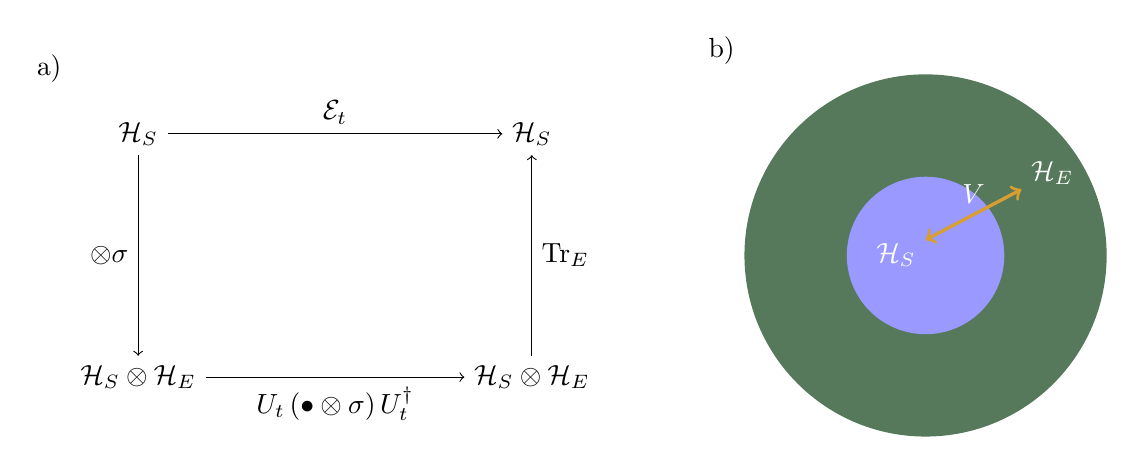
\begin{tikzpicture}%[transform canvas={scale=1.3}]
% Define colors
\definecolor{colorenv}{HTML}{55795A}
\definecolor{colorsys}{HTML}{7286D3}
\definecolor{colorarrow}{HTML}{D99E30}
  %%%%%%%%%%%%%%%%%5Commutation diagram
  % Define nodes
  \begin{scope}[local bounding box=drawA]
  \node (A) at (0cm,0) {$\mathcal{H}_{S}$};
   \node (B) at (5cm,0) {$\mathcal{H}_{S}$};
  \node (C) at (0cm,-3.09cm) {$\mathcal{H}_{S}\otimes\mathcal{H}_{E}$};
  \node (D) at (5cm,-3.09cm) {$\mathcal{H}_{S}\otimes\mathcal{H}_{E}$};
  % Draw arrows
   \draw[->] (A) -- (B) node[midway, above] {$\mathcal{E}_{t}$};
  \draw[->] (A) -- (C) node[midway, left] {$\otimes \sigma$};
  \draw[<-] (B) -- (D) node[midway, right] {$\mathrm{Tr}_{E}$};
  \draw[->] (C) -- (D) node[midway, below] {$U_{t}\left(\bullet\otimes\sigma\right)U_{t}^{\dagger}$};
\end{scope}
\node[above left] at (drawA.north west) {a)};
  \begin{scope}[local bounding box=drawB]
  %%%%%%%%%%The circles
  %Circles
  \fill[color=colorenv] (10cm,-1.545cm) circle (2.3cm);

  \fill[blue!40] (10cm,-1.545cm) circle (1cm);
  %Marks
  \node[text=white, anchor=east] (E) at (10cm,-1.545cm) {$\mathcal{H}_{S}$};
  \node[text=white, anchor=east] (F) at (12cm,-0.5cm) {$\mathcal{H}_{E}$};
   \draw[<->, line width=1.2pt, color=colorarrow, text=white] (E) -- (F) node[midway, above] {$V$};
  \end{scope}
 \node[above left] at (drawB.north west) {b)};
\end{tikzpicture}
\caption{Diagrams of the $S+E$ scheme. In a) the maps that define $\mathcal{E}_{t}$ are shown, and in b) a Venn-like diagram illustrating
the structure of the total system $S+E$, inspired in \cite{manzano2020short} }
\label{fig:SE_Diagrams}
\end{figure}

In figure (\ref{fig:SE_Diagrams}) two diagrams representing  the scheme are presented. On an intuitive level is true that any non-unitary
evolution should be of this form, nevertheless we provide a more axiomatic point of view to allow for a slight generalization and because in
practice it is not rarely possible to make progress with analytical methods using \eqref{eq:SE_map}. We demand from any physically aceptable
transformation the following:

\begin{itemize}
  \item Valid states are mapped into valid states.
  \item It is convex linear.
  \item  It should preserve the trace
\end{itemize}
The last two can be well motivated by considering a proper mixture of two ensembles of pure states i.e. with $N$ total copies, $\rho =
p_{1}\rho_{1} + p_{2}\rho_{2}$, applaying the given transformation $\mathcal{E}$ to the copies of  $\ketbra{\psi_{1}}$ and $\ketbra{\psi_{2}}$  must produce a new total ensemble with $p_{1}N$ copies of $\mathcal{E}(\ketbra{\psi_{1}})$ and $p_{2}N$ copies of
$\mathcal{E}(\ketbra{\psi_{2}})$ and the trace cannot change because then the state would be invalid. From this we introduce
\textit{\textbf{Completely Positive and Trace Preserving (CPTP)}} maps:

\begin{definition}
  Given two Hilbert Spaces $\mathcal{H}$ and $\mathcal{H}'$, a map $\mathcal{E}:\mathcal{L}(\mathcal{H})\to\mathcal{L}(\mathcal{H}')$ such that:
  \begin{enumerate}
          \item $\Tr{\mathcal{E}(\rho)}=\Tr{\rho}$ for all trace-class operators $\rho \in \mathcal{L}(\mathcal{H})$ (trace preserving)
          \item $\mathcal{E}(p_{1}\rho_{1}+p_{2}\rho_{2}) =p_{1}\mathcal{E}(\rho_{1})+p_{2}\mathcal{E}(\rho_{2}) $ for all $\rho_{1} \rho_{2} \in \mathcal{L}(\mathcal{H})$ and $p_{1}, p_{2} \geq 0$ s.t. $p_{1}+p_{2}=1$ (Convex linearity)
    \item if $\rho \in \mathcal{L}(\mathcal{H})$ is positive, then so is $\mathcal{L}(\rho)$ is also positive (positivity) and furthermore,
          for any linear extension to $\mathcal{L}(\mathcal{H}\otimes \mathcal{H}'')$ of the form $\mathcal{E}\otimes I''$ we have that
          $\mathcal{E}(\rho \otimes I)$ is also positive (complete positivity), where $\mathcal{H}''$ is any separable Hilbert space
          and $I''$ the identity on it.
  \end{enumerate}
  is called a \textbf{\textit{Quantum Channel}}.
\end{definition}
The last condition deserves a discussion as it did not appear directly in our motivation: mathematically it is a well known fact that there
exists maps $\mathcal{E}$ that send positive operator into positive operator yet their extensions fail to do so e.g. the transpose, so
to be consistent with the idea of \textit{sending states to states} one needs complete positivity;
to this one might argue that changing Hilbert Spaces is meaningless as it implies changing the underlying system of study, but there are of situations in which this is desirable e.g. initially a two level from which we will measure the energy of the photons produced in the energy
transitions, so it do is meaningful. A few key results for the manipulation of quantum channels are the following \cite{nielsen_quantum_2010,wiseman_quantum_2010, ,strasberg2022quantum}:

\begin{enumerate}
  \item There exists a Hilbert space $\mathcal{H}_{E}$, a state $\sigma$ in it and a unitary operator $U \in\mathcal{L}(\mathcal{H}_{S}\otimes\mathcal{H}_{E})$ such that $\mathcal{E}(\rho) = \Trp{E}{U\left(\rho\otimes\sigma\right)U^{\dagger}}$.
  \item There exists a set of operators $\{K_{j} \}_{j}$ such that $\mathcal{E}(\rho) = \sum_{j}\rho K_{j}^{\dagger}K_{j}$ and $\sum_{j}K_{j}K_{j}^{\dagger}=I$. These are called \textit{\textbf{Kraus Operators}}.
  \item Any map of the above forms is a quantum channel.
  \item The Kraus Operators representation of a quantum channel is not unique; any unitary combination is also a valid representation.
\end{enumerate}
The first one is what we already anticipated with the caveat that given an operation generically there is no unique way to implement it as
a $S+E$ scheme, the Kraus operators are in a lot of situations the main tool to manipulate these maps and suggest that we can
always implement a channel via the application of \textbf{\textit{Completely Positive Non-Trace Increasing (CP)}} maps  defined as $\mathcal{E}_{j}(\rho)=K_{j}\rho K_{j}^{\dagger}$ such that $\mathcal{E} = \sum_{j}\mathcal{E}_{j}$. This can be interpreted as an \textbf{\textit{stochastic map}} \cite{nielsen_quantum_2010} by the following
rewriting of the image of $\rho$:

\begin{equation}
  \mathcal{E}(\rho) = \sum_{j}\mathcal{E}_{j}(\rho) = \sum_{j}\Tr{\mathcal{E}_{j}(\rho)}\frac{\mathcal{E}_{j}(\rho)}{\Tr{\mathcal{E}_{j}(\rho)}},
\end{equation}

each $\frac{\mathcal{E}_{j}(\rho)}{\Tr{\mathcal{E}_{j}(\rho)}}$ is a valid density operator and $\Tr{\mathcal{E}_{j}(\rho)}\geq 0,
\sum_{j}\Tr{\mathcal{E}_{j}(\rho)}=1$ so we can say that when we apply the channel $\mathcal{E}$ there is a probability
$\Tr{\mathcal{E}_{j}(\rho)}$ of the output state being $\frac{\mathcal{E}_{j}(\rho)}{\Tr{\mathcal{E}_{j}(\rho)}}$. The main inconveniente
with this interpretation is the non-uniqueness of the possible output states unless one is using a particular physical platform that
defines them, nevertheless this is no surprise as in general we can not select such set of states from only a density operator. In figure
\ref{fig:stochastic_map_diagram} a drawing representing the idea is presented.
%%%%%%Stochastic Interpretation Quantum Channels
\begin{figure}[h]
  \centering
\begin{tikzpicture}[>=Stealth, thick]
    % Main box
    \draw (0,0) rectangle (6.5, 4.35);
       % Inner boxes and labels
    \node[draw, minimum size=0.5cm] (E0) at (4,3.5) {$\mathcal{E}_1$};
    \node[draw, minimum size=0.5cm] (E1) at (4,2.5) {$\mathcal{E}_2$};
    \node[draw, minimum size=0.5cm] (EN) at (4,0.5) {$\mathcal{E}_N$};
    % Dots for continuation
    \foreach \y in {1.8,1.5,1.2} {
        \draw[fill] (4,\y) circle (0.5pt);
    };
    % Input
    \node[minimum size=1.5cm, font=\Large] (input) at (-1,2.035)  {$\rho$};
    % First Intersection point
    \node (I0) at (1.0,2.035) {};
    % Arrow to the intersection
    \draw[-] (-0.7, 2.035) -- (1.0,2.035);
    %first vertical line
     \draw[-] (1.0,3.5)--(1.0, 0.5);
    %first horitonzal lines
    \draw[-] (1.0,3.5)--(E0) node[midway, above] {$\Tr{\mathcal{E}_{1}(\rho)}$};
    \draw[-] (1.0,2.5)--(E1) node[midway, above] {$\Tr{\mathcal{E}_{2}(\rho)}$};
    \draw[-] (1.0,0.5)--(EN) node[midway, above] {$\Tr{\mathcal{E}_{N}(\rho)}$};
    %Second intersection point
    \node (I1) at (6.0,2.035) {};
    %Second vertical line
    \draw[-] (6.0,0.5)--(6.0,3.5);
    %Horizontal lines
    \draw[-] (E0)--(6.0, 3.5) ;
    \draw[-] (E1)--(6.0, 2.5 ) ;
    \draw[-] (EN)--(6.0, 0.5) ;
    %Output
    \node[minimum size=0.5cm, font=\large] (output) at (8.3, 2.035) {$\mathcal{E}(\rho)$};
    %arrow out of the intersection
    \draw[-] (6.0,2.035)--(output);
    % caligraphic E below the big box
    \node[minimum size=0.5cm, font=\huge] (label) at (3, -0.5) {$\mathcal{E}$};
\end{tikzpicture}
\caption{Illustration of the stochastic map interpretation.}
\label{fig:stochastic_map_diagram}
\end{figure}

From here it is clear that weakening the trace preservation condition is desirable as we are interpreting each $\mathcal{E}$ also as
\textit{physical operations}. We end the section with the definition of a \textbf{\textit{Quantum Operation}} \cite{strasberg2022quantum,nielsen_quantum_2010,wiseman_quantum_2010}:

\begin{definition}
  Given two Hilbert Spaces $\mathcal{H}$ and $\mathcal{H}'$, a map $\mathcal{E}:\mathcal{L}(\mathcal{H})\to\mathcal{L}(\mathcal{H}')$ such that:
  \begin{enumerate}
          \item $\Tr{\mathcal{E}(\rho)}\geq\Tr{\rho}$ for all trace-class operators $\rho \in \mathcal{L}(\mathcal{H})$
          \item $\mathcal{E}(p_{1}\rho_{1}+p_{2}\rho_{2}) =p_{1}\mathcal{E}(\rho_{1})+p_{2}\mathcal{E}(\rho_{2}) $ for all $\rho_{1} \rho_{2} \in \mathcal{L}(\mathcal{H})$ and $p_{1}, p_{2} \geq 0$ s.t. $p_{1}+p_{2}=1$ (Convex linearity)
          \item is completely positive
  \end{enumerate}
  is called a \textbf{\textit{Quantum Operation}}.
\end{definition}
The results regarding equivalent representations can be generalized \cite{strasberg2022quantum,wiseman_quantum_2010}:
\begin{enumerate}
  \item There exists a Hilbert space $\mathcal{H}_{E}$, a state $\sigma$ in it, a unitary operator $U \in\mathcal{L}(\mathcal{H}_{S}\otimes\mathcal{H}_{E})$ and a  projector $P_{r}$ acting in $\mathcal{H}_{E}$ such that $\mathcal{E}(\rho) = \Trp{E}{P_{r}U\left(\rho\otimes\sigma\right)U^{\dagger}}$.
  \item There exists a set of operators $\{K_{j} \}_{j}$ such that $\mathcal{E}(\rho) = \sum_{j}\rho K_{j}^{\dagger}K_{j}$ and $\sum_{j}K_{j}K_{j}^{\dagger}\geq I$
  \item Any map of the above forms is a quantum operation.
  \item The Kraus Operators representation of a quantum operation is not unique; any unitary combination is also a valid representation.
\end{enumerate}
Conceptually operations are somewhat more desirable than channels yet they do not offer any considerable generalization as a set of operations
can always be completed into a channel \cite{nielsen_quantum_2010}. One last remark: due to the non-uniqueness of the decomposition into operations in a sense quantum channels are somewhat like black-boxes,
you know what goes in and what comes out yet unless you have extra information it is not possible to pin down exactly what happens inside the
channel.
\section{Generalized Measurements}
We have not addresed an important consistency question: are measurement collapses acceptable quantum operations? It is quickly to see that
in fact they are by defining the operation $\mathcal{E}_{r}(\rho)=P_{r}\rho P_{r}$ where $r$ is the eigenvalue of some observable and $P_{r}$ its
associated projector, this means that our formalism can really accomodate all the transformations required by the postulates. Without entering
directly into the phenomenology of measurements we can understand them with the following generic scheme: say we are perfoming an experiment
with $N$ possible outcomes indexed by ${r=1,..,N}$ just like in figure \ref{fig:stochastic_map_diagram}, each possible outcome corresponds to a
different collapse described by maps of the form $\mathcal{E}_{r}$ with a corresponding probability $\Tr{\mathcal{E}_{r}(\rho)}$ (Born rule).
It is possible to idenfity two different types of measurements: one when we known a measurement happend and which collapsed occured i.e.
the outcome of the experiment is known, this is  called  \textit{\textbf{a Selective Measurement}} \cite{diosi_short_2011}
and is described by:
\begin{equation}
\rho \to \mathcal{E}_{r}(\rho);
\end{equation}
and one in which all we known is that the experiment happened but not the outcome, this is called \textit{\textbf{a non-Selective Measurement}}
\cite{diosi_short_2011} and is described by

\begin{equation}
\rho \to \sum_{r}\mathcal{E}_{r}(\rho).
\end{equation}
So far the main physical assumption we have made is that our measurements are \textbf{\textit{Projective}} i.e. the post-measurement state
of a selective measuremente is given by projectors
\begin{equation}
\rho_{r} = \frac{P_{r}\rho P_{r}}{\Tr{P_{r}\rho}},
\end{equation}
but this doesn't have to be the case. Consider the following: no physical system $S$ might be directly measured as any measurement apparatus is
also a physical system $A$ which couples unitarily to $S$ in order to get correlated with it, and so it is debatable whether using the collapse postulate and the Born rule on $S$ is valid as the
result of the measurement really is read from the apparatus ... which itself must be measured by a second apparatus $A'$ and so on; this
potentially infinite chain of systems is called \textbf{\textit{a Von Neumann Chain}} and leaves us with the question of to which one should the
collapse postulate be applaied to; here we accept that using it on $A$ is already valid, hence the operation giving a selective measurement
should really be $\mathcal{E}_{r}(\rho) = \Trp{A}{P_{r} U\left(\rho\otimes\sigma \right)U^{\dagger}}$ where $U$ is the unitary evolution during
the coupling and $P_{r}$ a projector not on the Hilbert space of $S$ but of $A$ as the result is being read from it. We summarize this disscusion
in the following definition:

\begin{definition}
  Given a set of outcomes $r=1,2,3..$ and set of quantum operations  mapping the system to itself indexed by them $\{\mathcal{O}_{r}\}_{r=1}$  such that $\mathcal{O}=\sum_{r}\mathcal{O}_{r}$ is trace-preserving, we say that this is a \textit{\textbf{Generalized Measurement Scheme}}.
  We also define the following:
  \begin{enumerate}
    \item The probability of obtaining the result $r$ from a state $\rho$ is $\wp(r) = \Tr{\mathcal{O}_{r}(\rho)}$.
    \item The selective post-measurement state associated with the result $r$ is $\rho_{r} = \frac{\mathcal{O}_{r}(\rho)}{\Tr{\mathcal{O}_{r}(\rho)}}$.
    \item The non-selective post-measurement state is $\mathcal{O}(\rho)$.
  \end{enumerate}
\end{definition}
For a comprehensive treatment of generalized quantum measurements and its phenomenology the reader is refered to \cite{wiseman_quantum_2010}.
Finally, we analyze the expansion in Kraus operators of the probabilities in a generalized measurement scheme, the relevant concept
we will employ to study quantum estimation will come from this. Consider the operation associated with the result $r$, $\mathcal{O}_{r}$
and some set of Kraus operators associated with it $\{K\}_{rj}$, the probability of obtaining this outcome is from some state $\rho$ is:
\begin{equation}
  \wp(r) = \Tr{\left(\sum_{rj}K_{rj}^{\dagger}K_{j}\right)\rho}
\end{equation}
this tells us that really the probability is described by a single positive operator:
\begin{equation}\label{eq:sum_POVM}
\Pi_{r} = \sum_{rj}K_{rj}^{\dagger}K_{j},
\end{equation}
and it is clear that the trace-preserving condition imposes:
\begin{equation}\label{eq:sum_POVM}
\sum_{r}\Pi_{r} = I.
\end{equation}
From here comes the definition we have been trying to construct all along:

\begin{definition}
  A set of positive operators $\{\Pi_{r}\}_{r}$ such that $\sum_{r}\Pi_{r}=I$ is called \textit{\textbf{a Positive Operator Valued Measure (POVM)}}.
\end{definition}
The importance of POVMs is that in many cases, like the determination of a precision bound in  quantum estimation, only the probabilities of the outcomes are of interest; then defining a measurement scheme for this cases is not necessary as a POVM already induces the probabily distribution and describes them.

%%% Local Variables:
%%% mode: latex
%%% TeX-master: "../main"
%%% End:
